\section{Evaluation}
In this section, we present the evaluation results of proposed SaaS and IaaS controller and their impact on cloud based application
in terms of response time and energy consumption. The goal is to advocate the benefits
and limitations of each controller while experimenting
with real cloud application and real workload traces.

\subsection{Experimental setup}
\paragraph*{\textbf{Infrastructure configuration}}The experiments were conducted in Grid'5000 Lyon site,
with 3 physical machines linked by a 10 Gbit/s Ethernet
switch and connected to wattmeter. Each machine has two
2.3GHz Xeon processors (6 cores per CPU) and 16GB of
RAM, running Linux 2.6. Openstack Liberty was used
as platform, which requires one dedicated physical machine
for the cloud controller management system. Consequently,
the other physical machines were used as compute nodes to
host VMs, which in turn, are pre-configured to run Ubuntu
12.04.

\paragraph*{\textbf{Application Configuration}} We experimented with
RUBiS application \cite{rubis}, an eBay like auction site, which
is assumed to be a representative of popular e-commerce application 
and hence interactive web application. In Brownout \cite{brownout}, authors provided a user-to-user recommendation engine that is not core functionality of service but can enhance user experience. Along with that, we implemented a fairly simple item-to-item recommendation, to offer another level of user experience, which is showed at Listing 1. 

\begin{lstlisting}[language=SQL,caption={SQL statement for the recommender system.}, label={sql}]
SELECT
   items1.id
FROM
   items AS items1.id
   JOIN comments AS c ON items1.id = c.item_id
   JOIN items AS i2 ON items1.category = i2.category
 WHERE 
   i2.id = :current_item_id AND
   items1.nb_of_bids >= i2.item_id AND
   items1.id != :current_item_id
ORDER BY rating DESC
LIMIT 10;   
\end{lstlisting}


The
simple recommendation engine can be summarized as "Retrieve 10 products from same seller and same product category which has higher or same user bid count with high customer rating". Although both the
recommendation engines lack the sophistication and worldly complexities, they do
serve as a reasonable example of providing user experience that a cloud
application can isolate from core functionality of the service 
to activate or
deactivate at runtime. The recommendation is added
to the item visualisation page and to enable it, we defined
a function that reads a file, where actuator value is updated
in each control period and execute the associated modes for
each user request. For instance, Mode 1 activates the codes of
recommendation one, mode 2 activates both recommendations
and mode 0 provides no recommendation. Popular e-commerce providers provide multi-level recommendations to their users. Furthermore, the application is deployed with all its tiers \emph{i.e.,} web and database server inside a VM using a LEMP stack\footnote{\url{https://lemp.io/}}. Each application VM and Load-balancer (LB) VM were configured with 4 cores of CPU and 8GB of memory similar to Large flavor VM. Since, we used 2 compute servers, we could use maximum of 6 VM's and minimum at 2 VM's\footnote{1 LB VM and 1 application VM}. 

\begin{figure}[h]
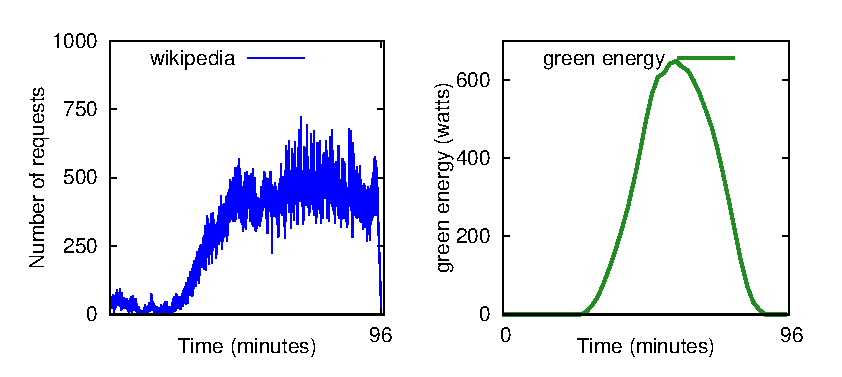
\includegraphics[scale=.7]{Graphs/workload_ucc.eps}
\caption{Workload trace}
\label{fig:workload} 
\end{figure}

\paragraph*{\textbf{Platform and Workload}} Our Proposed platform solution is hosted inside the cloud controller
machine. It monitors the 95th percentile response
time by aggregating the Nginx log of LB in each control period \emph{i.e.,} 20 seconds, whereas green energy
information is pushed by the infrastructure through an API in every 60 seconds. We have set $rt_{thr}$ 80\% and $decWorkPerc$ to 20\% at IaaS controller to evaluate our proposal.
We took the real traffic pattern of wikipedia german page of one day \cite{soodeh} and scaled the data set to fit with our experiment,
which is showed at Figure \ref{fig:workload}. 
To generate the workload, we used Gatling as load injector and choose an
open system model, where user requests are issued without
waiting for other users response from the system. 
Furthermore,
we emulated read-only workload where each user arrives to the homepage, browse any item category from a
vast catalog, click on a product to extract its information,
view seller rating and his/her reputation related to the
product. 
We traced the solar energy production that was added to
the grid for one day (12th April,2016) from EDF,
France\footnote{http://www.rte-france.com/fr/eco2mix/eco2mix} and scaled the
values suited for our experiment.
Furthermore, the duration
of each experiment was 96min and each was run several
times. We considered 96min as 24 hours, i.e., each 4min in
our experiments correspond to 1 hour.


\subsection{Consideration of delaying event}

\begin{figure} [htb]
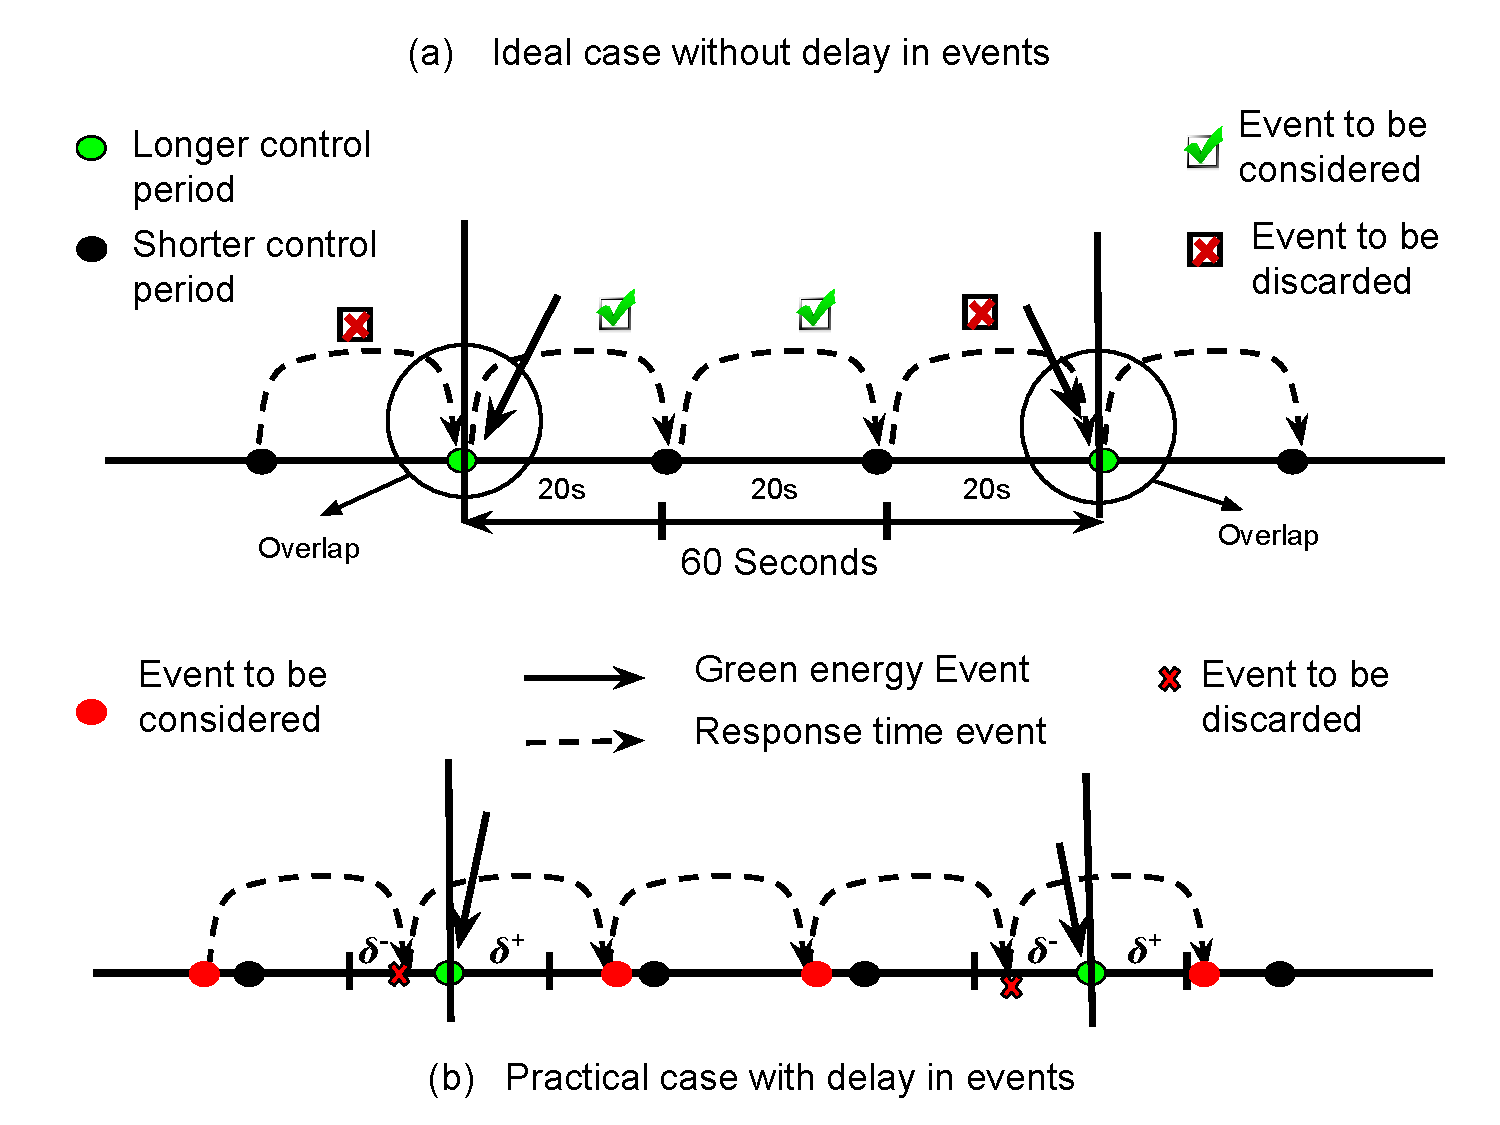
\includegraphics[scale=.35]{Graphs/implementation_UCC.pdf}
\caption{Algorithm implementation in detail}
\label{fig:implementation} 
\end{figure}

From Section \ref{saas-controller}, we see that, \emph{GE-C} controller has inner and outer loops which are activated in different time-scales and push events to the controller to make decision. In our experiments, outer (longer control period) and inner (shorter control period) loops are activated in each 60 seconds and 20 seconds respectively, which is showed in Figure \ref{fig:implementation}. Ideally, if both kind of events arrive without any delay, two different events will overlap each other. As our motivation is to maximize of green energy usage for \emph{GE-C} controller, we always make primary decision based on the green energy event pushed by IaaS by ignoring the response time event which is activated as inner loop, if both the event arrives concurrently. Concretely, it suggests that, between two big decision events in 60 seconds, we consider only two inner loop events and take actions if it is necessary indicated in Figure \ref{fig:implementation}(a).

But in case of delaying of any event, the scenario will not follow Figure \ref{fig:implementation}(a). As discussed before, the primary decision always depends on green energy event. Even though we receive response time event, no action is taken unless the system's response is high. Therefore, in case of delaying of response time event by micro to milliseconds, effects to the system remain almost unchangeable. In contrast, if the event delays by couple of seconds, for instance, inner loop event arrives just before or after the primary decision is made, it might affect the system dynamics to achieve the goal. To tackle the problem, we define a safety distance, denoted by $\delta^t$ to ensure that the controller does not take any action if response time event arrives in between "\textit{PrimaryDecision - $\delta^t$}" and "\textit{PrimaryDecision + $\delta^t$}". Figure \ref{fig:implementation}(b) illustrates the phenomena by an example. For our case, we choose safety distance as, $\delta^t$ = Time frequency of inner loop / $2$, which is equal to 10 seconds in our experiments.



\subsection{Results}

This section elaborately presents the results obtained during experiment at Grid'5000. We consider a baseline approach \emph{i.e.,} non-adaptive controller (NA), which lacks the capability of application adaptation and rely only on infrastructure adaptation based on response time.

%------------------------------------END-------------------------------------

\paragraph*{\textbf{Response time}}
\begin{figure} [htb]
\centering
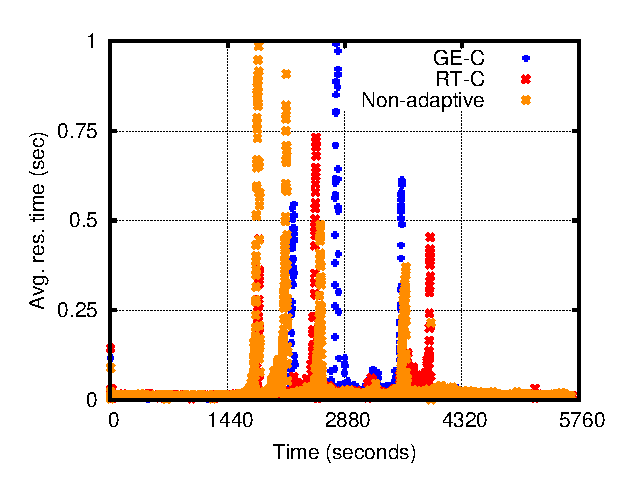
\includegraphics[scale=.8]{Graphs/responseTime.eps}
\caption{Response time incurred by Controllers}
\label{fig:rt}
\end{figure}
In Figure \ref{fig:rt}, we grouped response time by taking average over seconds. We kept response time set point as 1s. Since, our approach allows both level of adaptation depending on the changing environment, both RT-C and GE-C performed very closely by keeping 99th percentile response time around 274ms and 388ms. Figure \ref{fig:perc} shows the distribution of response time. Although, the baseline approach lacked application adaptation, it kept the 99th percentile response time around 500ms. On average, 3.7 million requests were injected during every experiment and only 7-20 requests failed for RT-C and 70-100 requests failed for GE-C. Therefore, both the controller ensure availability to five 9's (99.999\%).

%NA-.473
%GT-C-.388
%Rt-.274

\begin{figure} [htb]
\centering
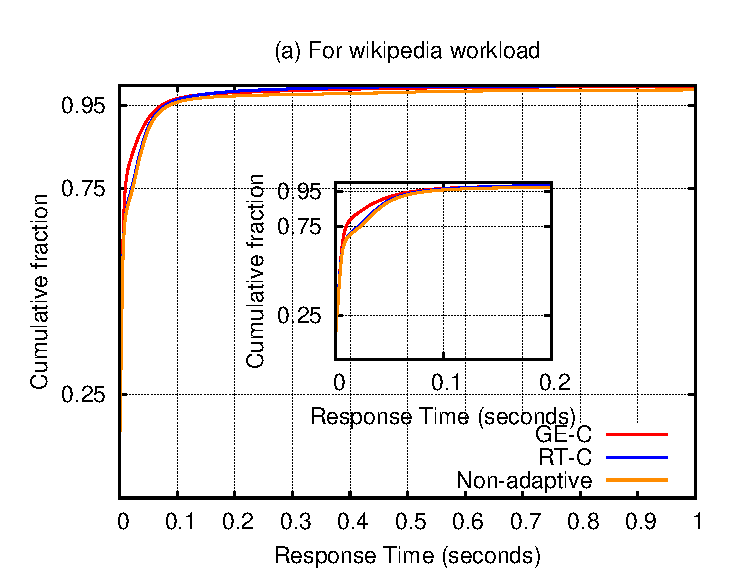
\includegraphics[scale=.75]{Graphs/percentile.eps}
\caption{Response time in percentiles}
\label{fig:perc}
\end{figure}





%----------------------------END-------------------------------------

\paragraph*{\textbf{Energy Consumption}}

In our experiment, each 4 minutes were considered as an
hour, thus we calculated the energy consumption of 24
hours, impacted by each controller, which is presented at
Table \ref{tab:watt1} and \ref{tab:watt2}. Each experiment was run several times and we found the energy consumption difference between each run
was 1$\sim$2 watts. At first, we scaled down the wikipedia workload to test the application controllers with static infrastructure, that is, in any given time application controllers were unable to use underlying elastic infrastructure. Table \ref{tab:watt1} summarizes that, GE-C can reduce brown energy consumption by 9.02\% and 6.4\% compared to NA and RT-C, while total energy consumption was reduced by 6.53\% and 6.4\% respectively. NA was supposed to consume more energy than RT-C since it lacks the capability to adapt application to lower level. Due to the heavy  user requests at some periods, NA approach saturated RUBiS application which was unable to accept any requests which resulted lower availability and lower energy consumption.

%Total: 5912.49
%Green: 3395.9
%Brown: 2516.59

\begin{table*}
\caption{Energy Consumption in Watts (Application adaptation)}
  \label{tab:watt1}
\begin{tabular}{cccl}
\toprule
Controller & Total Energy Consumption & Brown Energy Consumption & Green Energy Consumption\\
\midrule
Non-Adaptive & 3424.20 & 1934.66 & 1484.54 \\
RT-C & 3493.93 & 1975.18 & 1518.75  \\  %&1446.01 & 1941.32 & 3387.33 & --\\ \hline
GE-C & 3270.20 (NA > 6.53\%)(RT-C > 6.4\%) & 1760.09 (NA > 9.02\%) (RT-C > 10.88\%) & 1510.11 (NA < 1.2\%)\textcolor{red}{( RT-C > 0.50\%)} \\
\bottomrule
\end{tabular}
\end{table*}

%Rt & 3493.93 & 1975.18 & 1518.75  \\ \hline %&1446.01 & 1941.32 & 3387.33 & --\\ \hline
%Hybrid-Green & 3270.20 (6.4\%) & 1760.09 (10.88\%) & 1510.11 \alert{(0.50\%)} \\\hline

Afterwards, we proceeded with usual settings with the experiment having infrastructure elasticity capability for all the application controllers. Table \ref{tab:watt2} shows that, GE-C can reduce significant amount of brown energy by 35.11\% and 26.65\% compared to NA approach and RT-C respectively. Interestingly, RT-C consumed less green energy than the other application controllers, although this application controller was designed to consume more green energy than its counterpart application controllers. The reason being that, RT-C activated higher application mode  only in the presence of green energy, irrespective to the amount of user requests. Therefore, if the user requests are lower/higher while few green energy is available the controller activates medium service level mode (\emph{i.e.,} mode 1 which activates 1 kind of recommendation) and starts activating higher service level(\emph{i.e.,} mode 2 which activates 2 different kind of recommendation) when the amount of green energy increases. On the other hand, when green energy is scarce, application works at a low service level mode, that is, user can access the system but no recommendation is provided. In this experiment, the user requests started growing when green energy were scarce. Therefore, NA and RT-C both activated more application VMs than GE-C to cope up with the workload, which can be seen at Figure \ref{fig:vm}. Moreover, Figure \ref{fig:vm} shows that, GE-C followed green energy profile very closely while activating application Vms. It was possible due to fact that, we created green energy awareness to the application through \emph{GPaaScaler}. GE-C and RT-C both used maximum of 4 VM's while NA approach used 5 VM's for same workload.



\begin{table*}
\caption{Energy Consumption in Watts (Application and Infrastructure adaptation)}
  \label{tab:watt2}
\begin{tabular}{cccl}
\toprule
Controller & Total Energy Consumption & Brown Energy Consumption & Green Energy Consumption\\
\midrule
Non-Adaptive & 5912.49 & 2516.59 & 3395.9 \\
RT-C & 5574.78 & 2226.16 & 3348.62  \\  %&1446.01 & 1941.32 & 3387.33 & --\\ \hline
GE-C & 4796.17 (NA > 18.88\%)(RT-C > 13.96\%) & 1632.77 (NA > 35.11\%) (RT-C > 26.65\%) & 3163.4 \textcolor{red}{(NA > 6.83\%)( RT-C > 5.53\%)} \\
\bottomrule
\end{tabular}
\end{table*}

\begin{figure} [htb]
\centering
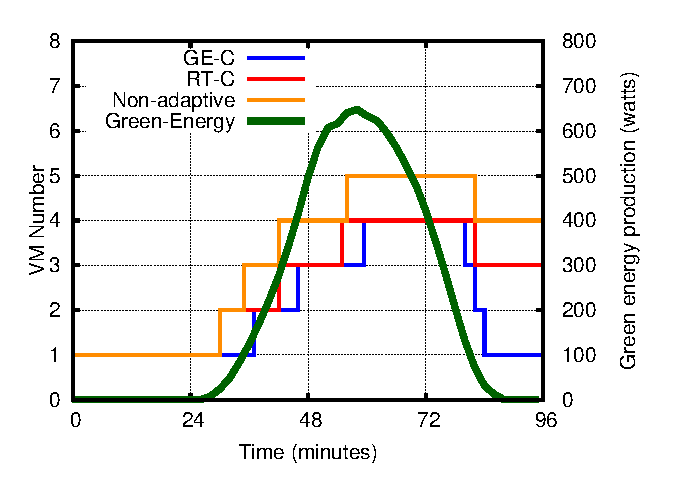
\includegraphics[scale=.8]{Graphs/vm.eps}
\caption{Number of VM usage during experiment}
\label{fig:vm}
\end{figure}

%----------------------------------END-------------------------------------

%0 Non-adaptive 8.748
%1 RT-C 6.696 (23.45 %)
%2 GE-C 5.508 (37.03 %) (21.568 %)

\paragraph{\textbf{Cost analysis}}

Since, our proposed GPaaScaler architecture is agnostic to infrastructure provider and type, it can be plugged on top of public cloud infrastructure. Therefore, we wanted to validate how much each application controller would cost with same application and workload profile. Since, we used large flavor VM's, we fixed instance costs to 0.104\textdollar/hour. Since, we considered 4 minutes of duration to 1 hour in our experiment, we calculated the amount of instances and their duration throughout the experiment. We considered partial time spent in the experiment as full instance hour. Figure \ref{fig:cost} shows the cost incurred by all the application controller. GE-C incurred 37.03\% and 21.56\% lesser cost than NA approach and RT-C.

\begin{figure} [htb]
\centering
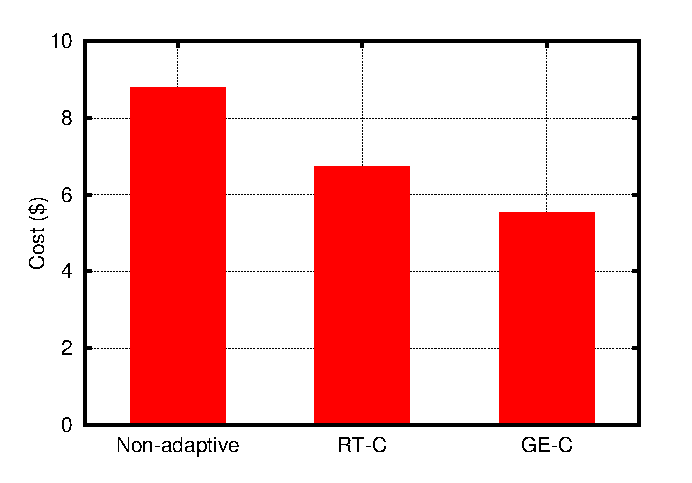
\includegraphics[scale=.7]{Graphs/cost.eps}
\caption{Cost analysis for VM usage}
\label{fig:cost}
\end{figure}

\section{Discussion}



